\chapter{Product}\label{chap:product}

\section{Implementation of the prototype}

\section{Programming language choice}

% TODO: Table of languages

\subsection{Functional programming paradigms}

% PHP vs Clojure

\subsection{Web programming with functional languages}

% Similarities to JavaScript (and it's popularity)

\section{Prototype rewrite in LISP}

\section{Persistent storage}
\subsection{Yet Another Protein Schema}

\section{Search engine design}

%%%%%%%%%%%%%%%%%%%%%%%%
%% Query tree diagram %%
%%%%%%%%%%%%%%%%%%%%%%%%

\begin{figure}[t]
\centering
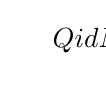
\begin{tikzpicture}
\tikzset{level distance=50pt, sibling distance=1.5pt}
  \Tree [.{$Q$}
    [.{$id$} ]
    [.{$N$}
      [.{$Q$}
        [. \node(q0){$q_0$}; ]
        [. \node(qn){$q_n$}; ]
      ]
      [.{$A$}
        [. \node(a0){$a_0$}; ]
        [. \node(an){$a_n$}; ]
      ]
      [. {$N$}
        [. \node(n0){$n_0$}; ]
        [. \node(nn){$n_n$}; ]
      ]
      [.{$eq$} ]
    ]
    [.{$P$}
      [.{$P$}
        [.{$p_l$} ]
        [.{$p_h$} ]
      ]
      [.{$M$}
        [.{$m_l$} ]
        [.{$m_h$} ]
      ]
      [.{$E$}
        [.{$e_0$} ]
        [.{$e_1$} ]
        [.{$e_2$} ]
        [.{$e_3$} ]
      ]
      [.{$L$}
        [.{$l_s$} ]
        [.{$l_l$} ]
      ]
      [.{$F$}
        [.{$f_n$} ]
        [.{$f_s$} ]
      ]
    ]
    [.{$E$}
      [.{$m$} ]
      [.{$T$}
        [. \node(tl){$t_l$}; ]
        [. \node(th){$t_h$}; ]
      ]
    ]
  ]
\begin{scope}[dashed]
\draw (a0)--(an);
\draw (n0)--(nn);
\draw (q0)--(qn);
\end{scope}
\end{tikzpicture}
\caption[Structure of the query tree for composing searches]
        {Structure of the query tree used for composing searches of
          the PIP-DB dataset. Leaf nodes represent properties. Nodes
          with an uppercase name denote compound AND conditionals.}
\label{fig:query-tree}
\end{figure}

%%%%%%%%%%%%%%%%%%%%%%%%
%% Query tree listing %%
%%%%%%%%%%%%%%%%%%%%%%%%


\lstset{language=Lisp}
\begin{center}
\begin{lstlisting}[label=lst:query-tree,caption={
      [Clojure implementation of the query tree]
      Implementation of the query tree in Clojure, from the file
      \texttt{query.clj}. Note the flat query hierarchy and the
      use of the \texttt{for} macro for expanding multivalued
      queries.}]
    (AND
     (EQ   {:field "id"            :value id :exact true})
     (for [word q]
       (EQ {:field "Protein-Names" :value word}))
     (for [word q_any]
       (EQ {:field "Protein-Names" :value word}))
     (for [word q_ne]
       (NE {:field "Protein-Names" :value word}))
     (EQ   {:field "Protein-Names" :value q_eq})
     (EQ   {:field "Source"        :value q_s})
     (EQ   {:field "Location"      :value q_l})
     (EQ   {:field "Method"        :value m})
     (EQ   {:field "Sequence-Name" :value seq})
     (GTE  {:field "real_pi_min"   :value pi_l})
     (LTE  {:field "real_pi_max"   :value pi_h})
     (GTE  {:field "real_mw_min"   :value mw_l})
     (LTE  {:field "real_mw_max"   :value mw_h})
     (GTE  {:field "real_temp_min" :value t_l})
     (LTE  {:field "real_temp_max" :value t_h})
     (EQ   {:field "real_ec1"      :value ec1 :numeric true})
     (EQ   {:field "real_ec2"      :value ec2 :numeric true})
     (EQ   {:field "real_ec3"      :value ec3 :numeric true})
     (EQ   {:field "real_ec4"      :value ec4 :numeric true}))
\end{lstlisting}
\end{center}

\subsection{Incorporating BLAST+ searching}

\subsection{Design of an API for searching services}

% RESTFUL API

\section{Performance and security}

\section{Usage instructions}
